% SPDX-License-Identifier: CC-BY-SA-4.0
% Author: Matthieu Perrin
% Part: 
% Section: 
% Sub-section: 
% Frame: 

\begingroup

\begin{frame}[fragile]{Que peut-on observer ?}

  \vspace{-25mm}
  \begin{lstlisting}[gobble=4]
    class Caches {
      static int (*\Structure{x = 0,}  \Alert{y = 0;}*)
      public static void main(String args[]) {
        new Thread(() -> {
          (*\Structure{x = 1;}*)
          System.out.println( (*\Alert{y}*) );
        }).start();
        new Thread(() -> {
          (*\Alert{y = 1;}*)
          System.out.println( (*\Structure{x}*) );
        }).start();
      }
    }
  \end{lstlisting}

  \uncover<2>{
    \onBlock[right=.42\textwidth, y=10mm]{Architectures UMA\\ (Uniform Memory Access)}{
      \centering
      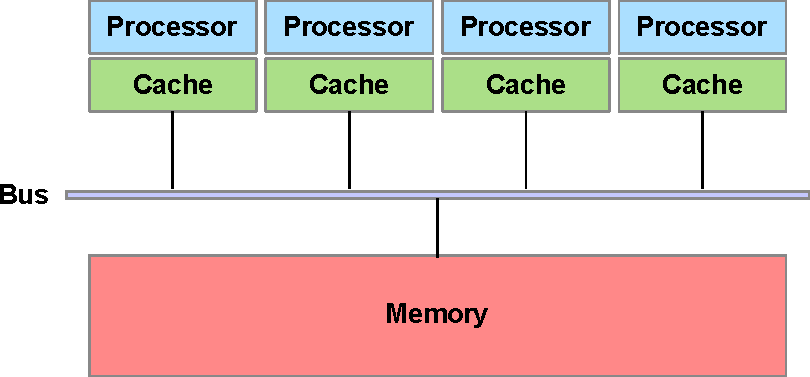
\includegraphics[height=1.8cm]{uma}
    }
    \onExampleBlock[y=-15mm]{Mot-clé \lstinline{volatile int x;} (depuis Java 5)}{
      \begin{itemize}
      \item Tout le cache est invalidé \structure{avant chaque lecture}  de $x$
      \item Tout le cache est invalidé \structure{après chaque écriture} de $x$
      \item Le cache n'est pas invalidé \structure{pendant} une lecture ou écriture de $x$ 
      \end{itemize}
    }
    \onAlertBlock[y=-35mm]{Attention}{
      \begin{itemize}
      \item Une invalidation de cache est très inefficace !
      \end{itemize}
    }
  }
  
\end{frame}

\endgroup
\endinput
